\documentclass[12pt, a4paper]{article}
\usepackage[turkish]{babel}
\usepackage[utf8]{inputenc}
\usepackage{graphicx}
\usepackage{amsmath}
\usepackage{multirow}

\usepackage[inner=2.5cm, % Inner margin
			outer=3cm, % Outer margin
			bindingoffset=0.5cm, % Binding offset
			top=2.5cm, % Top margin
			bottom=3cm, % Bottom margin
]{geometry}
\graphicspath{ {./pics/} }
\newcommand{\HRule}{\rule{\linewidth}{0.8mm}}


\pagenumbering{roman}
\begin{document}

\begin{titlepage}


\centering

\textsc{\LARGE İSTANBUL TEKNİK ÜNİVERSİTESİ}\\[0.5cm]% Name of your university/college
\textsc{\LARGE FİZİK MÜHENDİSLİĞİ}\\[1.5cm]
\textsc{\large Bitirme Projesi}\\[0.5cm]% Minor heading such as course

\HRule \\[0.4cm]
{ \huge \bfseries KONU} % Title of your document
\HRule \\[1.5cm]

\begin{minipage}{0.4\textwidth}
\begin{flushleft} \large
\emph{Öğrenci:}\\
Ömer Faruk KADI % Your name
\end{flushleft}
\end{minipage}
~
\begin{minipage}{0.4\textwidth}
\begin{flushright} \large
\emph{Danışman:} \\
Doc. Dr. Ahmet Levent Subaşı % Supervisor's Name
\end{flushright}
\end{minipage}\\[2cm]

{\large 2021-2022 GÜZ}\\[2cm] 

\begin{figure}[ht!]
    \centering
    \shorthandoff{=}
    
\includegraphics[width=0.5\textwidth]{itu-logo1.jpg}
\end{figure}

\vfill % Fill the rest of the page with whitespace
\end{titlepage}

\tableofcontents
\thispagestyle{empty}



%----------------------------------------------------------------------------------------------
\newpage
\setcounter{page}{1}
\addcontentsline{toc}{section}{Özet}
\begin{abstract}


\end{abstract}
%----------------------------------------------------------------------------------------------
\newpage
\addcontentsline{toc}{section}{Teşekkür}
\section*{\centering Teşekkür}
%----------------------------------------------------------------------------------------------
\newpage
\pagenumbering{arabic}
\setcounter{page}{1}
\section{Giriş}

\subsection{Satır İçerisinde Denklem}

\hspace{1cm}Satır içerisinde denklem \( x^n + y^n = z^n \) bu şekilde yazılabilir.

\subsection{Numarasız Denklem}

\hspace{1cm}Numarasız denk şu şekilde yazılabilir.

\begin{equation*}
E=mc^2 
\end{equation*}

\subsection{Numaralı Denklem}

\begin{equation} \label{eq1}
i\hbar \frac{\partial}{\partial t}\Psi(\mathbf{r},t) = \hat H \Psi(\mathbf{r},t)
\end{equation}

Numaralı denklemlere (\ref{eq1}) yazı içinde bu şekilde referans verilebilir.

\subsection{Çok Satırlı Denklem}

\hspace{1cm} Çok satırlı denklem bu şekilde yazılabilir.

\begin{multline*}
p(x) = 3x^6 + 14x^5y + 590x^4y^2 + 19x^3y^3 +  2y^6 - a^3b^3\\ 
- 12x^2y^4 - 12xy^5 + 2y^6 - a^3b^3
\end{multline*}



\subsection{Tablo Ekleme Ekleme}
\hspace{1cm} Ayrıntılı bir tablo bu şekilde eklenebilir. Yazı içerisinde tabloya Tablo \ref{table:1} bu şekilde referans verilebilir.

\begin{table}[h!]
\centering
\begin{tabular}{ |p{3cm}||p{3cm}|p{3cm}|p{3cm}|  }
\hline
\multicolumn{4}{|c|}{Ana Başlık} \\
\hline
Başlık 1& Başlık 2 &Başlık 3&Palşık 3\\
\hline
Parametre 1  	& değer 	&değer	&değer\\
Parametre 2	& değer  	&değer	&değer\\
Parametre 3	& değer 	&değer	&değer\\
Parametre 4	& değer 	&değer	&değer\\
Parametre 5	& değer 	&değer	&değer\\
Parametre 6	& değer  	&değer	&değer\\
Parametre 7	& değer 	&değer	&değer\\
\hline
\end{tabular}
\caption{Tablo hakkında açıklama}
\label{table:1}
\end{table}

\subsection{Görsel Ekleme}
\hspace{1cm} İlgili görsel bu şekilde eklenebilir. Yazı içerisinde görsele Şekil \ref{fig:test} bu şekilde referans verilebilir. 

\begin{figure}[h!]
 	\centering
	\shorthandoff{=}
      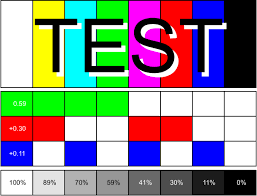
\includegraphics[width=0.7\textwidth]{Test.png}
	\caption{\label{fig:test}Şekil ile ilgi açıklama}
\end{figure}

\subsection{Bir Makaleye Referans Verme}
Herhangi bir makaleye \cite{als} bu şekilde referans verilebilir.

%----------------------------------------------------------------------------------------------
\newpage
\section{Sonuç}

%----------------------------------------------------------------------------------------------
\newpage
\addcontentsline{toc}{section}{Kaynaklar}
%\bibliographystyle{mnras.bst}
\bibliographystyle{plain}
\bibliography{biblio.bib}




\end{document}
